\chapter{光谱仿真与纹影诊断}
	TDLAS测量的前提是选择合适的吸收谱线：要求线强适中、温度敏感且无干扰。同时，由于TDLAS测量的是视线积分信号，必须通过Abel反演才能恢复径向参数分布。因此，光谱仿真和反演算法是测量的两个基础环节。本章首先介绍HITRAN光谱仿真与波段优选，然后介绍Abel反演算法的开发与验证，以及FSR波长标定方法，最后给出纹影诊断的实验结果。
	\subsection{CO$_2$吸收光谱仿真}
	基于HITRAN数据库（2020版）和line-by-line模型，对CO$_2$在中红外波段的吸收光谱进行系统仿真。HITRAN数据库提供了分子吸收谱线的线强、低态能量、展宽系数、配分函数等关键参数，line-by-line模型则逐条计算各谱线的吸收贡献并叠加。仿真覆盖了本课题实验工况的温度范围（200--300~K）和压力范围（0.03--0.5~MPa），重点考察CO$_2$吸收峰的温度灵敏度、线强大小以及H$_2$O干扰峰的叠加程度。仿真程序基于Python实现，核心步骤：
	\begin{enumerate}[label=(\arabic*)]
		\item 从HITRAN数据库提取谱线参数（线强、低态能量、展宽系数等）；
		\item 计算Voigt线型（WHV算法）叠加各谱线贡献；
		\item 输出吸光度$A(\nu)=\sum_i S_i(T)\phi_i(\nu) n_{\rm CO2}L$，其中$S_i$为线强，$\phi_i$为Voigt线型，$n_{\rm CO2}$为CO$_2$数密度，$L$为光程。
	\end{enumerate}
	图\ref{fig:h2o_co2_compare}给出了中红外波段在1~bar压力、1~cm吸收光程条件下，H$_2$O与CO$_2$吸收光谱的全波段对比。
	\begin{figure}[H]
		\centering
		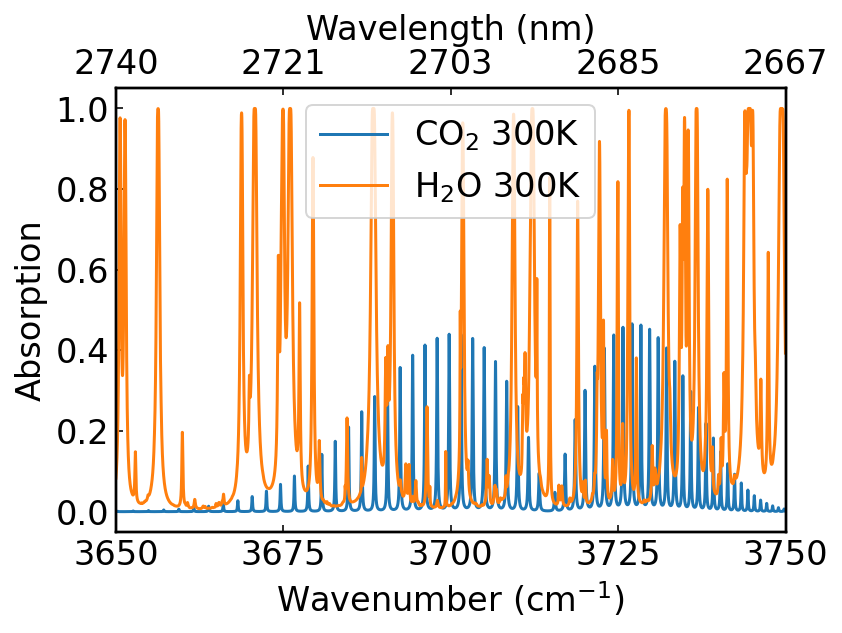
\includegraphics[width=0.85\textwidth]{figures/fig11.png}
		\caption{中红外波段1~bar条件下吸收距离1~cm水和二氧化碳吸收对比}
		\label{fig:h2o_co2_compare}
	\end{figure}
	仿真结果表明：在2.7~$\mu$m波段（$\tilde{\nu} \approx 3696~\text{cm}^{-1}$）附近，CO$_2$吸收线强适中（$S \approx 10^{-21}~\text{cm}^{-1}\text{molecule}^{-1}\text{cm}^2$），温度灵敏度高（$d\ln S/dT \approx 2.5\%/\text{K}$），且与H$_2$O干扰峰的谱线分离度大于$0.5~\text{cm}^{-1}$，因此确定为最佳实验波段。这一选择的核心物理依据在于：2.7~$\mu$m波段CO$_2$吸收谱线的低态能量差异较大（约几百至一千波数），使得不同谱线对温度的响应敏感度不同，为双线测温法提供了足够的温度灵敏度。相比之下，4.2~$\mu$m波段虽然线强更大，但低态能量普遍偏低，温度灵敏度仅有约1.0\%/K左右，且该波段CO$_2$吸收信号受环境背景（空气中约420~ppm CO$_2$）的严重干扰，不适合低温射流测量。2~$\mu$m波段线强较弱，温度敏感性不足，同样不适合本实验。
	综合对比全中红外波段（2.7~$\mu$m、2~$\mu$m、4.2~$\mu$m），筛选标准：
	\begin{itemize}
		\item 吸收线强适中（峰值吸光度0.1-0.5），避免饱和或信号过弱；
		\item 线强温度灵敏度$d\ln S/dT$尽可能大；
		\item H$_2$O干扰吸收峰分离度$>0.5$~cm$^{-1}$；
		\item 避开CO$_2$谱线重叠区域。
	\end{itemize}
	图\ref{fig:selected_band}给出了选定波段在3694--3700~cm$^{-1}$范围内的局部放大图，可见CO$_2$在该波段存在多条独立的特征吸收峰，而H$_2$O吸收峰数量极少且强度微弱（约两个数量级以下），谱线分离度良好。
	\begin{figure}[H]
		\centering
		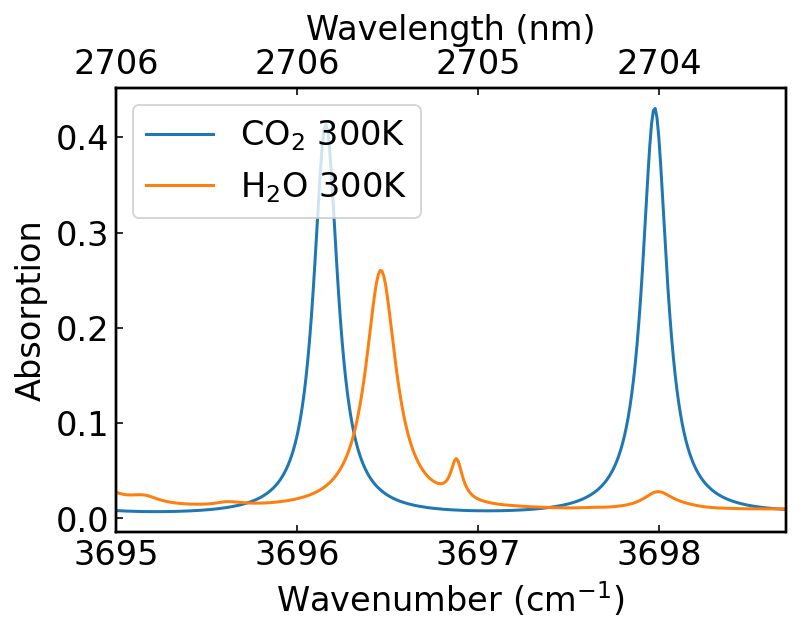
\includegraphics[width=0.85\textwidth]{figures/fig12.png}
		\caption{2.7~$\mu$m波段1~bar条件下水和二氧化碳吸收对比（局部放大）}
		\label{fig:selected_band}
	\end{figure}
	谱线对的具体筛选遵循以下原则：（1）两条谱线相距不超过5~cm$^{-1}$，以避免波长扫描范围过大导致的非线性效应；（2）两条谱线的低态能量差$\Delta E''$尽可能大（以增强温度灵敏度），一般要求$\Delta E'' > 500$~cm$^{-1}$；（3）两条谱线的线强在同一量级，避免信号动态范围过大；（4）无H$_2$O、N$_2$O等常见气体的交叉吸收干扰。基于以上原则，最终选取3694.3~cm$^{-1}$和3696.2~cm$^{-1}$两条相邻谱线作为测温谱线对，两者的低态能量差约660~cm$^{-1}$，在200--300~K温度范围内双线强度比变化约2.5倍，满足测量精度要求。
	仿真所得吸收峰形（峰位、峰高、半高宽）与后续激光器出厂测试报告、实验示波器波形完全吻合（峰位偏差$<0.02$~cm$^{-1}$，半高宽偏差$<5\%$），验证了仿真模型的可靠性。
	\subsection{FSR波长标定方法}
	TDLAS实验采集的信号以采样点数为横坐标，需转换为波数域。采用标准具（Thorlabs SA200-12B，镜间距1.5~cm，FSR=0.333~cm$^{-1}$，精细度$F=200$）进行波长标定。
	标定步骤：
	\begin{enumerate}[label=(\arabic*)]
		\item 将标准具串联在激光器与测试光路之间，分束片（透反比90:10）将10\%激光导入标准具；
		\item 无射流条件下采集标准具透射信号（图\ref{fig:fsr_signal}），获取等间隔干涉峰序列；
		\item 以空气中残留CO$_2$在3696.0~cm$^{-1}$的吸收线为绝对波数基准；
		\item 识别各干涉峰序号$m$与对应采样点位置$i_m$，线性拟合$i_m=i_0+k\cdot m$；
		\item 建立采样点-波数映射关系：
		\begin{equation}
			\nu(i)=\nu_{\rm ref}+\mathrm{FSR}\times\frac{i-i_{\rm ref}}{\Delta i}
			\label{eq:fsr}
		\end{equation}
		其中$\nu_{\rm ref}$为参考峰波数，$i_{\rm ref}$为参考峰采样点，$\Delta i$为相邻干涉峰间采样点间隔。
	\end{enumerate}
	\begin{figure}[H]
		\centering
		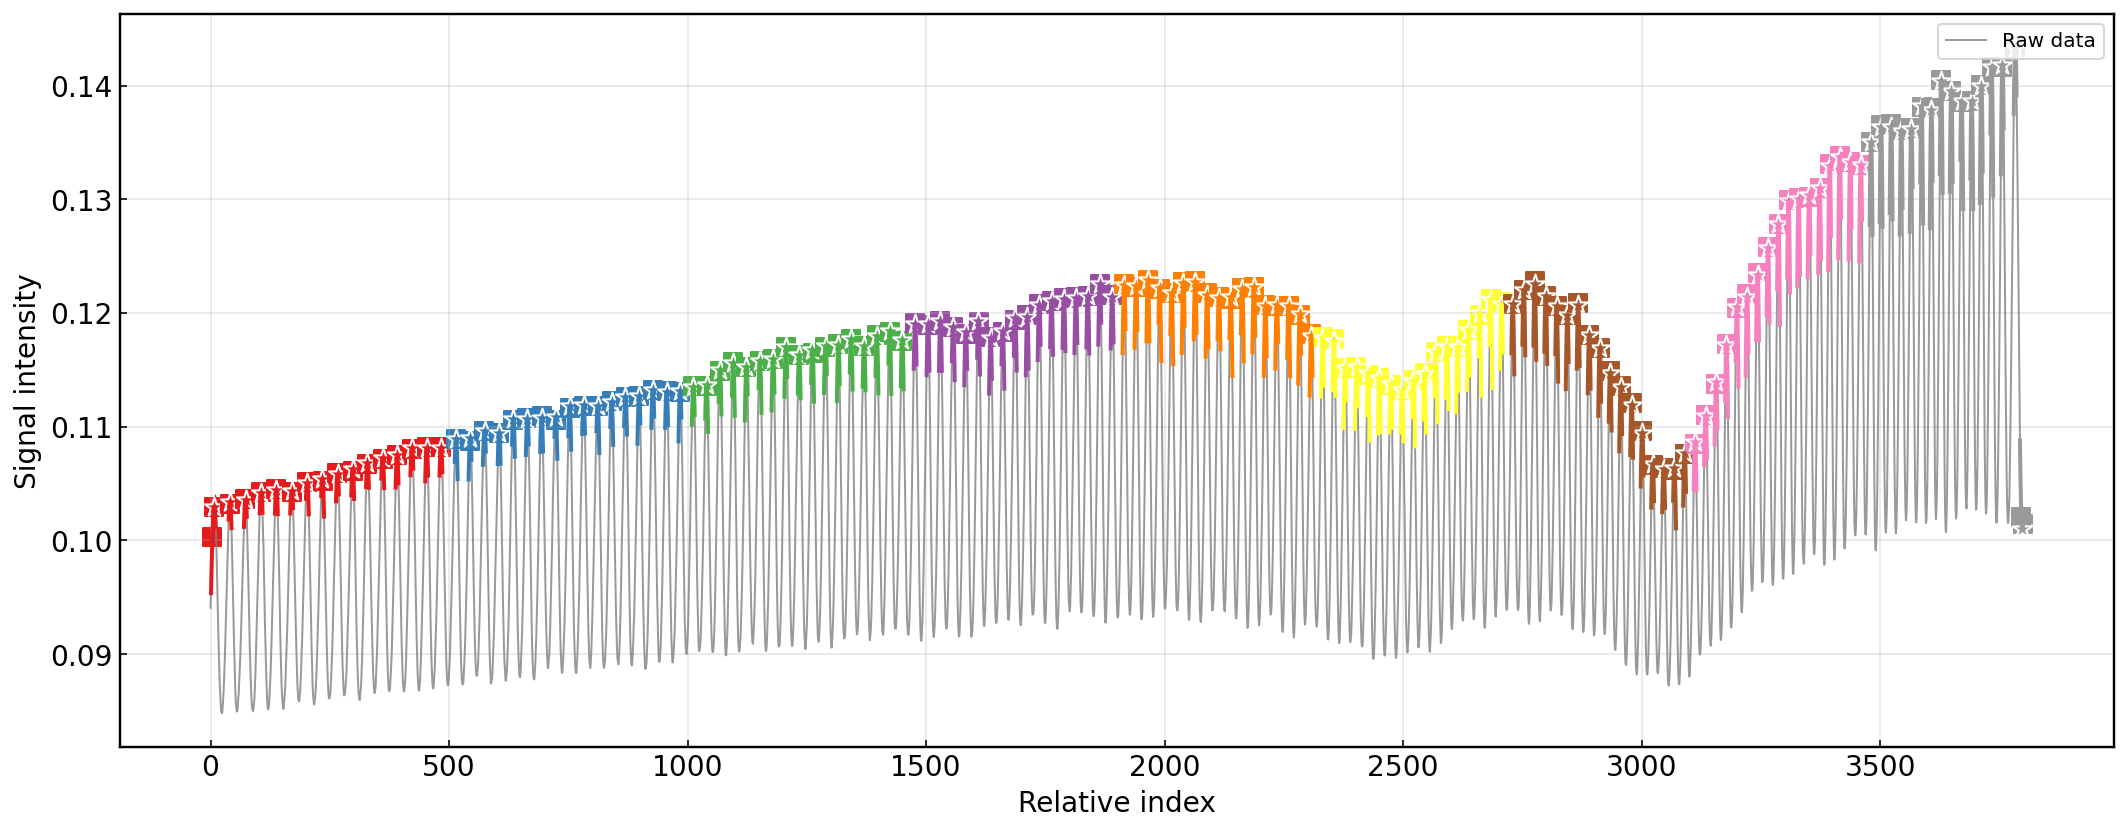
\includegraphics[width=0.8\textwidth]{figures/fig9.png}
		\caption{FSR干涉峰图（用于波长标定）}
		\label{fig:fsr_signal}
	\end{figure}
	标定完成后，用已知波长的其他CO$_2$吸收线验证标定精度。当前标定存在微小偏移（约0.01-0.02~cm$^{-1}$），怀疑为峰值检测算法误差，需后续修正。
	\subsection{Abel反演算法开发与验证}
	对于轴对称流场（图\ref{fig:abel_geometry}），TDLAS测量的线积分信号与径向参数分布满足Abel积分方程：
	\begin{equation}
		p(x)=2\int_{x}^{R}\frac{f(r)r}{\sqrt{r^{2}-x^{2}}}\,dr
		\label{eq:abel}
	\end{equation}
	其中$p(x)$为视线偏移距离$x$处的线积分信号，$f(r)$为径向坐标$r$处的参数值，$R$为流场半径。
	\begin{figure}[H]
		\centering
		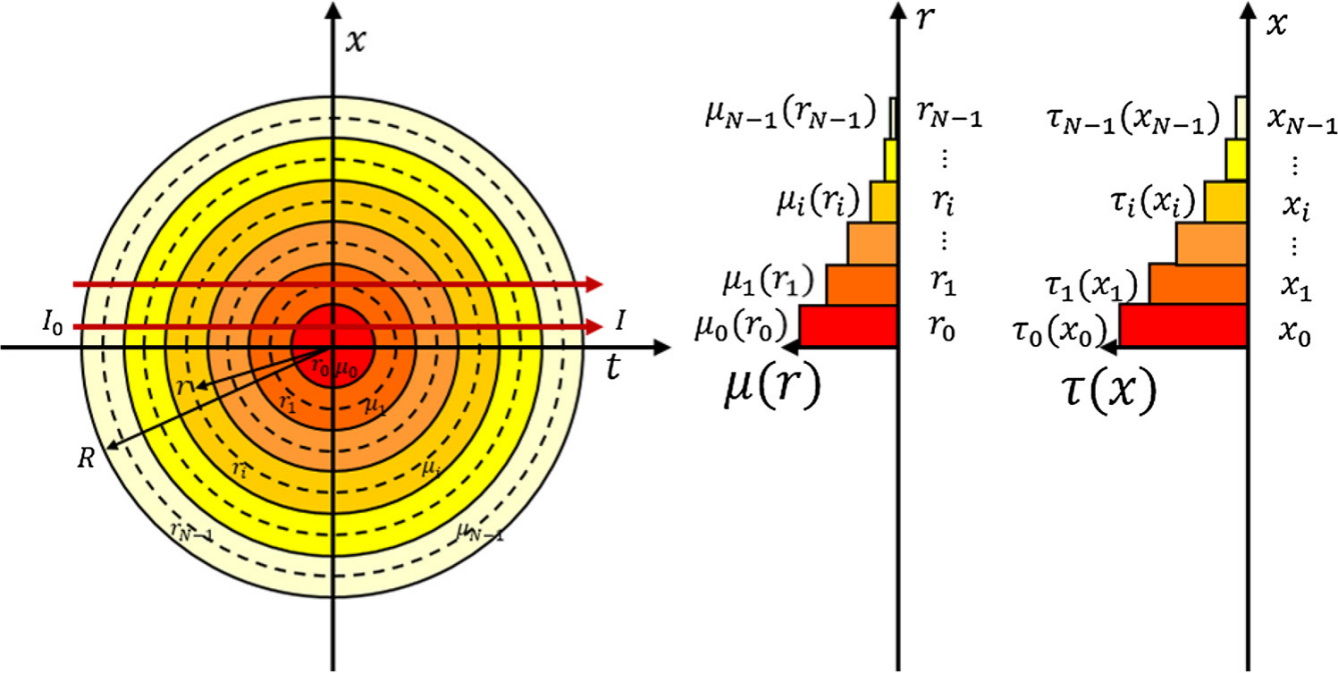
\includegraphics[width=0.5\textwidth]{figures/fig10.png}
		\caption{轴对称流场Abel变换几何示意}
		\label{fig:abel_geometry}
	\end{figure}
	本工作实现了三种反演算法：
	\subsubsection{两点法}
	离散公式：
	\begin{equation}
		f(r_j)=-\frac{1}{\pi}\sum_{i=j}^{N-1}\frac{p(x_{i+1})-p(x_i)}{\sqrt{x_{i+1}^2-r_j^2}}
		\label{eq:twopoint}
	\end{equation}
	对投影数据光滑性要求高，噪声敏感。
	\subsubsection{三点法}
	基于拉格朗日插值，使用三个相邻投影点计算斜率：
	\begin{equation}
		f(r_j)=-\frac{1}{\pi}\sum_{i=j}^{N-1}w_i\cdot\frac{p(x_{i+1})-p(x_{i-1})}{x_{i+1}-x_{i-1}}\cdot\frac{1}{\sqrt{x_i^2-r_j^2}}
		\label{eq:threepoint}
	\end{equation}
	其中$w_i$为权重系数。三点法对噪声抑制优于两点法。
	\subsubsection{洋葱剥皮法}
	从外向内逐层反演：最外层环带$j=N$，$f(r_N)=p(x_N)/(2\Delta r)$；然后逐层用投影差分减去已反演部分贡献：
	\begin{equation}
		f(r_j)=\frac{p(x_j)-2\sum_{k=j+1}^{N}f(r_k)\sqrt{r_k^2-r_j^2}\Delta r}{2\Delta r}
		\label{eq:onion}
	\end{equation}
	为评估三种反演算法的精度和抗噪能力，构建高斯解析场$f(r)=300\exp(-r^2/(2\sigma^2))$（$\sigma=5$~mm，$R=10$~mm），按式(\ref{eq:abel})正向投影。高斯场是对轴对称射流径向参数分布的合理近似，能够模拟射流中心峰值高、向边缘平滑过渡的典型特征。在投影数据中加入1\%、3\%、5\%高斯白噪声，每种噪声水平重复10次蒙特卡洛模拟，以统计反演误差的分布特征。
	三种算法的基本原理如下：\textbf{两点法}直接利用相邻两条视线信号的差分反演局部吸收系数，运算简单但本质上对噪声敏感，因为差分运算会放大高频噪声；\textbf{三点法}利用三个相邻点的信息进行局部插值后再差分，相当于对数据进行了前置平滑，具有一定的噪声抑制能力；\textbf{洋葱剥皮法}从最外层开始逐层剥离，将每层吸收信号扣除后推向内层，物理直观但误差会逐层向中心累积。
	图\ref{fig:abel_2point}—\ref{fig:abel_onion}给出了加入3\%噪声后三种算法的反演结果与真值的对比。
	\begin{figure}[H]
		\centering
		\includegraphics[width=0.85\textwidth]{figures/fig13.png}
		\caption{3\%噪声条件下两点法重建结果}
		\label{fig:abel_2point}
	\end{figure}
	\begin{figure}[H]
		\centering
		\includegraphics[width=0.85\textwidth]{figures/fig14.png}
		\caption{3\%噪声条件下三点法重建结果}
		\label{fig:abel_3point}
	\end{figure}
	\begin{figure}[H]
		\centering
		\includegraphics[width=0.85\textwidth]{figures/fig15.png}
		\caption{3\%噪声条件下洋葱剥皮法重建结果}
		\label{fig:abel_onion}
	\end{figure}
	误差统计（除对称轴附近5\%区域，该区域因Abel变换本身的奇异性容易发散）：
	\begin{itemize}
		\item \textbf{无噪声}：三种算法均$<1\%$，说明在理想条件下三种方法均能高精度恢复原始场；
		\item \textbf{1\%噪声}：两点法2.3\%，三点法1.8\%，洋葱剥皮法2.1\%，三种方法性能接近；
		\item \textbf{3\%噪声}：两点法12.5\%（边缘$>15\%$），三点法4.2\%，洋葱剥皮法6.8\%，两点法因差分放大了噪声而显著恶化，三点法的局部平滑特性显现优势；
		\item \textbf{5\%噪声}：三点法8.5\%，洋葱剥皮法12.3\%，两点法失效（边缘误差$>30\%$）。
	\end{itemize}
	三点法在3\%噪声条件下整体误差约4.2\%，且无尖峰发散，表明其在实际实验测量（信噪比通常在20--40之间，对应噪声约2.5\%--5\%）中具有最佳的鲁棒性。综合考虑精度、鲁棒性和计算效率，确定三点法为实测数据核心反演算法。
	\subsection{温度反演方法}
	采用双线强度比法（Two-line thermometry），基于玻尔兹曼分布模型。原理如下：
	对于光学薄气体，积分吸光度与谱线强度成正比：
	\begin{equation}
		I_i(r)=\int_{\Delta\lambda_i} A(r,\lambda)d\lambda = \frac{N(r)L}{\ln 10}S_i(T(r))
		\label{eq:integrated_absorbance}
	\end{equation}
	取两条谱线的积分吸光度之比：
	\begin{equation}
		R(r)\equiv\frac{I_1(r)}{I_2(r)}=\frac{S_1(T(r))}{S_2(T(r))}
		\label{eq:ratio}
	\end{equation}
	谱线强度随温度变化满足：
	\begin{equation}
		S(T)=S(T_{\rm ref})\frac{Q(T_{\rm ref})}{Q(T)}
		\exp\left[-c_2E''\left(\frac{1}{T}-\frac{1}{T_{\rm ref}}\right)\right]
		\frac{1-\exp(-c_2\nu/T)}{1-\exp(-c_2\nu/T_{\rm ref})}
		\label{eq:st}
	\end{equation}
	其中$c_2=hc/k\approx1.438777$~cm$\cdot$K，$Q(T)$为配分函数，$E''$为低态能量。将式(\ref{eq:st})代入式(\ref{eq:ratio})，得到温度$T$满足的非线性方程：
	\begin{equation}
		F(T)=\frac{S_1(T)}{S_2(T)}-R(r)=0
		\label{eq:temp_solve}
	\end{equation}
	采用牛顿迭代法求解（初值$T_0=300$~K，收敛阈值$10^{-6}$）。谱线选取标准：
	\begin{itemize}
		\item 低态能量差$|\Delta E''|>500$~cm$^{-1}$，保证温度灵敏度；
		\item 两谱线互不重叠，与相邻线分离度$>0.2$~cm$^{-1}$；
		\item 线强适中，确保实验信噪比SNR$>20$。
	\end{itemize}
	\subsection{纹影诊断结果}
	完成铝型材框架试验台（200$\times$120$\times$100~cm）的组装与调试。图\ref{fig:setup_photo}为实验台实物照片。
	\begin{figure}[H]
		\centering
		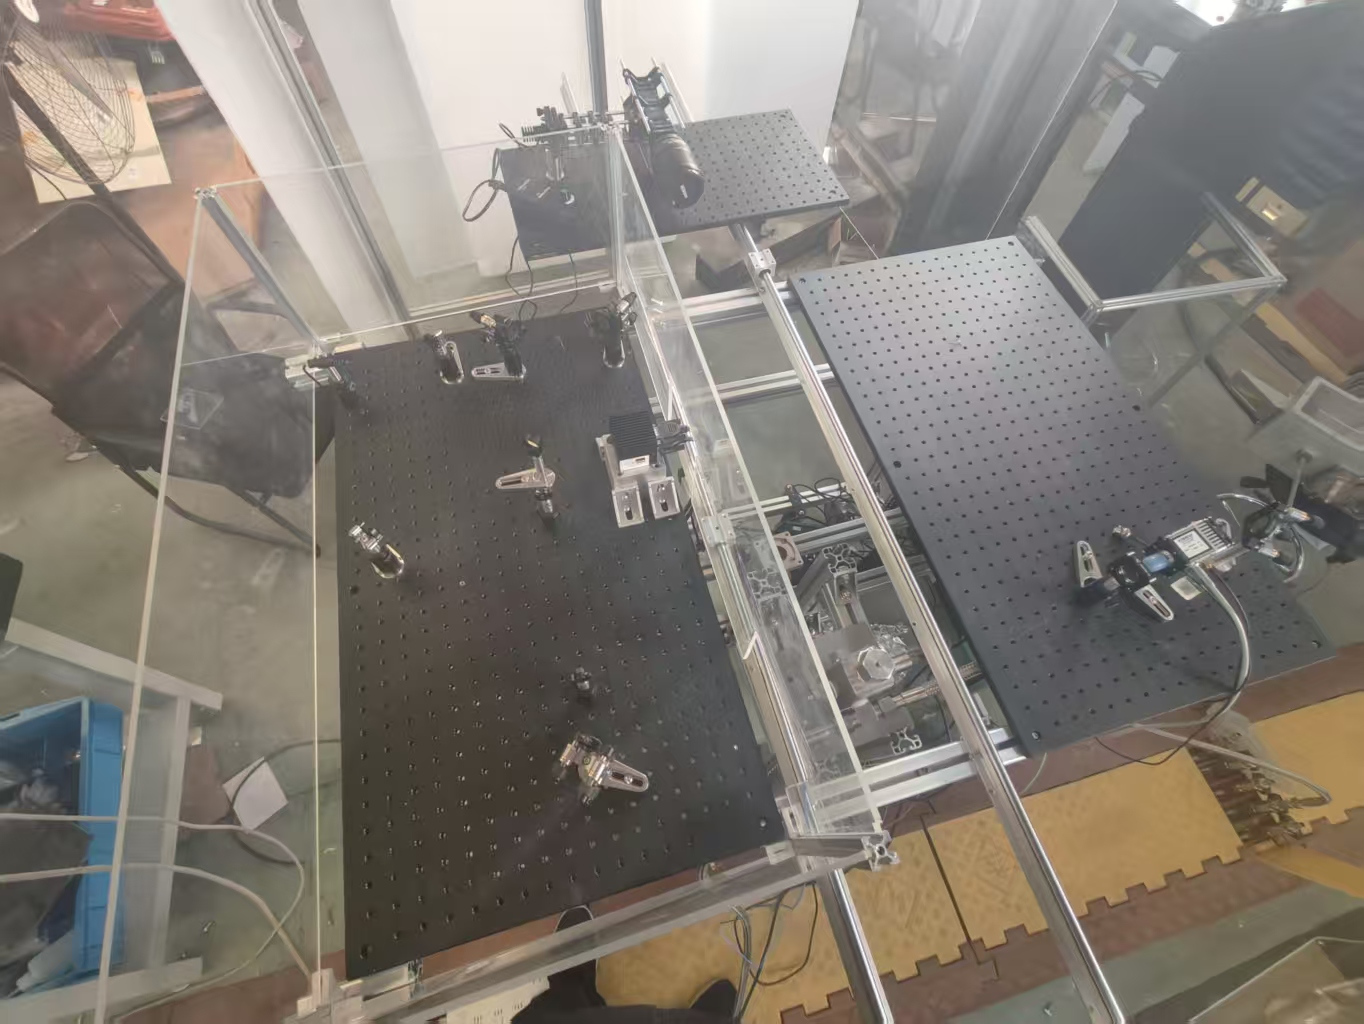
\includegraphics[width=0.7\textwidth]{figures/fig16.png}
		\caption{射流试验台实物照片（含气路、腔体、位移平台）}
		\label{fig:setup_photo}
	\end{figure}
	混合腔体气密性测试：关闭所有阀门后通入CO$_2$至0.6~MPa，10分钟内压力从0.600~MPa降至0.595~MPa（下降0.005~MPa/min），满足实验要求（$<$0.01~MPa/min）。
	纹影系统成功拍摄不同上游压力下的射流结构。图\ref{fig:schlieren_result}给出了0.5~MPa、1~mm喷嘴条件下的纹影图像。
	\begin{figure}[H]
		\centering
		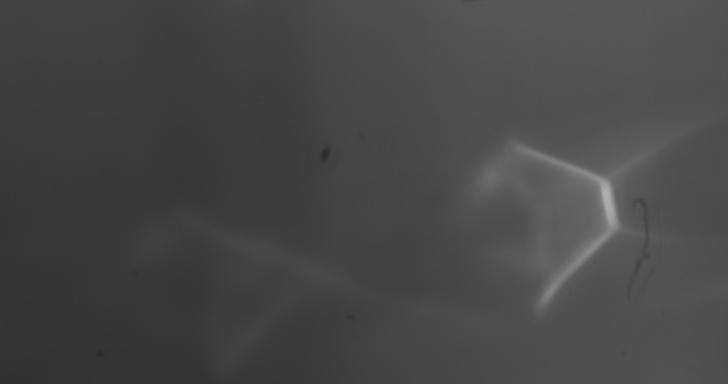
\includegraphics[width=0.7\textwidth]{figures/fig17.png}
		\caption{纹影图像（上游压力0.5~MPa，1~mm喷嘴）}
		\label{fig:schlieren_result}
	\end{figure}
	马赫盘距喷嘴出口约2.8~mm，与Fluent仿真值（3.0~mm）偏差$<10\%$，射流边界清晰，验证了射流系统的可重复性。
	\subsection{分析与讨论}
	\begin{itemize}
		\item \textbf{波段选择的物理依据}：2.7~$\mu$m波段的高温度灵敏度来源于该波段CO$_2$分子振动-转动跃迁的低态能量差异较大。双线测温法的基本原理是$\ln(R) = -\frac{\Delta E''}{k_B T} + \ln\left(\frac{A_2 S_2(T_0)}{A_1 S_1(T_0)}\right)$，其中$R$为两条谱线的强度比，$\Delta E''$为两条谱线的低态能量差。$\Delta E''$越大，$\ln R$随$T$的变化率越大，即温度灵敏度越高。本课题选取的3694.3~cm$^{-1}$与3696.2~cm$^{-1}$谱线对$\Delta E'' \approx 660$~cm$^{-1}$，在低温区间（200--300~K）的测温灵敏度约为2.5\%/K，即1~K温度变化对应约2.5\%的强度比变化，完全满足实验需求。
		\item \textbf{反演算法选择的理论依据}：三点法的优势在于利用三个相邻点的信息进行二次插值，相当于对数据进行了局部平滑，天然具有一定的噪声抑制能力。而从信息论的角度看，三点法利用了三个点的信息进行局部重建，实际上等价于对原始离散数据进行了一次低通滤波，其截止频率与采样间距和局部曲率相关，能有效压制高频噪声。相比之下，两点法直接用相邻点差分，在波数域上相当于乘以$2i\sin(\pi f \Delta r)$，高频分量被显著放大，因此对噪声极其敏感。
		\item \textbf{仿真与实验的衔接}：HITRAN仿真提供谱线参数和温度灵敏度，Fluent仿真提供流场温压范围的真值，两者共同为实验设计和数据处理提供依据。具体而言：HITRAN仿真的作用在于确定最优测量波段和谱线对，并预先计算出各工况下的理论吸收光谱形态；Fluent仿真的作用在于确定射流的空间尺度（半宽约1--2~mm）和参数变化范围，为采样点数量（径向6点）和扫描范围（0--5~mm）提供依据；Abel反演验证的作用在于确认在目标信噪比条件下（本系统约22倍，对应噪声4.5\%），三点法能够保证$<5\%$的重建精度。
	\end{itemize}
	\subsection{本章小结}
	（1）通过HITRAN数据库line-by-line仿真系统分析了中红外波段CO$_2$与H$_2$O的吸收光谱特征，确定2.7~$\mu$m（3696~cm$^{-1}$）为最佳实验波段。该波段CO$_2$线强适中（$10^{-21}$量级），温度灵敏度高达2.5\%/K，且H$_2$O干扰峰的谱线分离度大于$0.5$~cm$^{-1}$，谱线对的$\Delta E'' \approx 660$~cm$^{-1}$保障了低温区间（200--300~K）的测温精度。仿真峰形与出厂测试报告及实验波形吻合（峰位偏差$<0.02$~cm$^{-1}$，半高宽偏差$<5\%$）。
	（2）通过高斯解析场加噪测试，系统对比了三种反演算法的精度和抗噪性能。两点法对噪声敏感（3\%噪声下误差12.5\%），洋葱剥皮法存在误差累积效应（3\%噪声下误差6.8\%），三点法结合局部插值与噪声抑制优势，在3\%噪声条件下误差4.2\%且无尖峰发散，确定为实测数据核心反演算法。
	（3）纹影系统成功捕捉马赫盘结构，位置与Fluent仿真偏差$<10\%$，验证了射流系统的可靠性。
	（4）建立了“HITRAN光谱仿真$\to$Fluent流场仿真$\to$Abel正演投影$\to$加噪反演验证$\to$误差定量评估”的完整方法链，验证了从仿真到实验的整套数据处理流程的可靠性，为后续实测数据的处理提供了方法论基础和误差界限参考。
	% ==================== 第五章 层析扫描实验与温度分布 ====================

